\documentclass{sigplanconf}
\usepackage{amsmath}
\usepackage[pdftex]{graphicx}
\begin{document}
\special{papersize=8.5in,11in}
\setlength{\pdfpageheight}{\paperheight}
\setlength{\pdfpagewidth}{\paperwidth}

\conferenceinfo{Compiler Project '13}{Dec 12, 2013, Balcksburg, VA, USA}
\copyrightyear{2013}
\copyrightdata{978-1-nnnn-nnnn-n/yy/mm}
\doi{nnnnnnn.nnnnnnn}

\titlebanner{banner above paper title}        % These are ignored unless


\title{FDO Based Inlining in LLVM}
\subtitle{A Dynamic Optimization Techniqe}

\authorinfo{Arijit Chattopadhyay}
           {Viriginia Tech}
           {arijitvt@vt.edu}
           
\authorinfo{Nabanita Maji}
           {Virginia Tech}
           {nabanita@vt.edu}

\maketitle

\begin{abstract}
Feedback Directed Optimization (aka FDO) is a very promising compiler optimization technique. This has been well adapted in gcc but LLVM lacks an efficient FDO based inlining mechanism. Our optimization technique autmatically instruments a program, creates a trace and then determines the factors for the optimal build and finally generates the build for maximum performance w.r.t. execution time. The entire framework consists of the 4 independent modules. This method gives on an average 1.6\% run time improvement and more than 9\% runtime improvement for mutator programs.
\end{abstract}

\terms
Compilers, Optimization

\keywords
Feedback-directed, Cross-module, Function Inlining.

\section{Introduction}
Most of the compiler optimization techniques are based on the static analysis of the code. Static analysis works on the module level granularity, which corresponds to a file. During the static analysis of the code, it is very difficult to correctly determine the most frequently taken path. Programming languages like C, C++, which supports the source code to be distributed across multiple source files, it is impossible to know the details of the callee function at the compile time. However at the link time the linker has the information about the declaration of every function. So our implementation tries incorporate those information of the link time and the runtime and provide them back at the compile time to generate an optimized built.
\paragraph{•} Inlining is a technique in which  programs are optimized by reducing the function call overhead and copying the source code of the callee into the caller function. For an example in \ref{inl_exp} , \emph{doCal} in \emph{a.c} calls \emph{calculate} in \emph{b.c} for 10000 times. This incurs good amount of function call overhead on the system. If we can build a framework which copies the source of  \emph{calculate} into \emph{doCal}  function, then we can get good performance benefit.  However there is a clear case of size increase is happening here.  This size increase may also affect the performance. With increase in instruction count, program incurs the pressure on the instruction cache during execution. This demands an efficient system, which can find out the trade-off between the size increase to the performance benefit and create the build accordingly.
\paragraph*{•} In this technical report, we are going to present the details of our new Feedback Directed Optimizations based on dynamic analysis technique. Next part of the paper has been organised in the following way, 
	\begin{itemize}
		\item We will first discuss some background and the previous work done in this domain.
		\item Next, we will discuss the design and the implementation details of our transformation and analysis opt passes, which serve various purposes, from trace generation to the final compilation.
		\item Then we will move on to the result of our experiments followed by the conclusion and possible future extension.
	\end{itemize}
Our noble approach is completely automated and highly modular.

\begin{figure}
\label{inl_exp}
\begin{center}
	 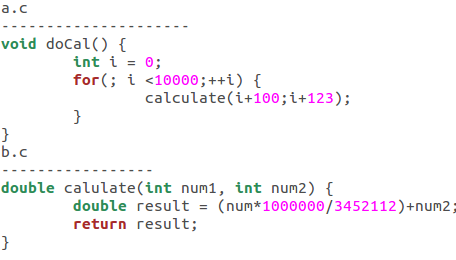
\includegraphics[width =80mm, height=45mm]{inlining.png} 
\end{center}
\caption{Inlining by an example}
\end{figure}

\section{Background}
Feedback directed optimization technique is very well established in \emph{gcc} compiler \cite{Li} and \cite{lipo} . \emph{LLVM} also has some inline techniques established like \textit{always\_ inline} and \textit{simple\_ inline} but they are very primitive implementation and does not use any FDO based information or dynamic analysis of the source code.
\paragraph*{•} In traditional FDO based inlining technique in gcc, Cross Module Optimization (CMO) and FeedBack Directed Optimization(FDO) are coupled together. Since procedure boundary most of the time acts as a limiting factor to various optimization,Li\cite{Li} has moved the optimization strategy beyond the function boundaries. Moving the optmization technique beyond the process boundary is also being discussed in \citep{Triant}.
\paragraph*{•} Combining these two approaches in LLVM, has been used in the Google commercial compilers \cite{diego}. Probably \cite{diego} is the most closest work to us.  In their approach they used \emph{Auto FDO}, which does not need any training run and requires external trace file to generate the dynamic information needed for the compiler optimization. In order to learn, they do not need multiple training runs. As per our best knowledge, details of their work is not available except some outline slides.
\paragraph*{•} In this work, we are also generating a trace file from the instrumented IR of the target program and develop a dynamic call graph of the frequency count and based on that knowledge we are building the optimal build of a program. The details of the design in being discussed in the next section.

\section{Design and Implementation}

	\paragraph{•}
	Our implementation of feedback directed inlining consists of multiple stages primarily implemented as different transformations in llvm. The trace generation transformation can be applied to any intermediate representation to instrument it to generate trace files when run on sample input. The details of the implementation is explained in the next subsection. The trace is analysed by analysers implemented as scripts  to determine the optimal threshold value for tuning the extent of inlining. The threshold values once calculated can be fed into the inliner which is another LLVM transformation pass.  The inliner decides on which functions to inline based on certain parameters ( as explained in subsequent sections) and inlines them. The loop detection pass is a helper pass run on the intermediate representation to identify the functions containing loop within them.  
\subsection{Trace Generation}
	The first step of a feedback directed inlining is generating the execution sequence. In order to generate the  trace of execution sequence of an application\' s binary, the binary needs to be instrumented such that at runtime it generates its own footprints. The instrumentation on an applications executable was achieved in our implementation by running a LLVM pass on its intermediate representation (aka IR) file. Since, the motive of our trace-generation is profiling the runtime behaviour and using it as a feedback for inliner, we are interested only in function calls. From this trace another module generates the weighted dynamic callgraph. The edges of this dynamic callgraph is annotated with the frequency of execution of that particular edge during runtime. An edge of a callgraph is said to be executed whenever a function call happens from one node of the edge to another in the direction of the arc. These annotated call graph gives us the information of the hot paths in call graph , which we use in our inlining heuristics to determine which functions are viable candidates for inlining. Details of trace generation process can be found in Trace Generation diagram.\ref{TraceGen}.
	\begin{figure}
	 \begin{center}
		 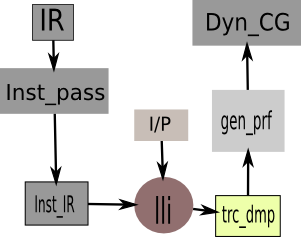
\includegraphics[width=50mm,height=30mm]{design.png} 
	 \end{center}
	 \caption{Trace Generation Process}
	 \label{TraceGen}
 \end{figure}
    \paragraph*{•}
    The LLVM pass is implemented to instrument the intermediate representation file, inserts a function call before each callsite in the IR. When the instrumented binary is run on a sample input, this injected callsite calls a function in our profile generation framework. This function takes the caller and callee as input and uses it to build and maintain the dynamic callgraph in its datastore which also updates the frequency of calls from a particular caller to  a particular callee, whenever it is encountered more multiple times during runtime. At the exit point of he instrumented binary, the dynamic callgraph generated at this execution is dumped into the trace file.
    
    	\subsection{Trace analysis}
	A single or multiple trace files may be gene­­rated by the first stage depending on number of different inputs we are providing to the instrumented test program. We examined that the trace files generated by our test suites and realised that the call frequencies in the trace file tend to clutter around certain ranges. The distribution of the call frequencies suggested that it is possible to derive a optimal frequency threshold. To do so we implement a basic analyser script.which reads the call frequencies from the trace file and classifies them. The classifier counts the number of call frequencies present in a particular range (bucket) and increments the counter of the bucket.For our implementation we use a fixed size bucket of  1000. After the classification phase we analyse the cardinality of each bucket and chose the most populated bucket. Once the appropriate bucket is identified, we consider multiple values at regular intervals inside the bucket and use them as frequency thresholds for inlining and measure the performance improvement. For e.g. in our case , the bucket size being 1000, we perform 10 iterations at an interval of 100 starting form the lower range of the bucket. We consider the iteration that gives the highest performance benefit and use that particular value as threshold.
	We calculated our optimal threshold using our analyser and verify its accuracy by gathering performance values on multiple thresholds. Our test results verify that the threshold provided by our analyser is acceptably close to the frequency threshold that gave us the highest performance \ref{src_ana}.
	\subsection{Loop detection}
	 Inlining eliminates the call overhead of a function. But if the call overhead of the function is negligible compared to execution time of the same function, the benefits of inilining are very less in those cases. Functions containing loops tend to have a higher execution time. Hence our implementation considers functions with loops as a non-viable candidates for inlining. This pass detects all the functions that has loops in it and dumps them into a separate file which is read by the inliner's filter. Any function mentioned in the file will not be inlined by the inliner. Execution of this pass is recommended but optional. 	
	\subsection{Inlining}	
    In this phase we determine which are candidates for inlining. There are two major factors which contribute to this decision, viz.
    \begin{itemize}
        \item Frequency of the Callee function at the CallSite.
        \item Instruction Count of the Callee function.
    \end{itemize}
    These two information we gather from the dynamic call graph generated from the trace of the instrumented code \ref{TraceGen}.

    \paragraph{} In order to maintain the call frequency, we have implemented a map which holds the FDO data and provides us the frequency for each call instruction at a callsite. The map has the Caller and Callee name amalgamated together as a key and the frequency as the value. By querying this map we determine one of the decisive factor for inlining. If the frequency and the instruction count of the callee is below a threshold limit then we decide that the callee function could be candidate for inlining. The threshold limit is also dynamically calculated based on the result of the \textit{Analyzer} discussed in the previous section. Over inlining also harms performance. If we inline many functions it eventually increases the code size to a great extend. Over inlining increases instruction count and as a matter of fact, that creates huge overhead on the instruction cache. As a result program runs much slower compared to its non-lined version. So carefully choosing theses parameters is the key to the success of this approach.
    \paragraph{}However even if a candidate pass the above criteria, it may not suitable for inlining always. There are some terminal cases, which we need to consider before actually determining the candidate. For that purpose, we have implemented a filter, which can check these terminal cases. This filter does not permit inlining for the following cases.
	\begin{itemize}
		\item Candidates which are recursive
		\item Functions containing \textit{no\_ inline} attribute
		\item Candidates having external library linkage
        \item It is not possible to inline the callee structure.
        \item Callee function has loop.
	\end{itemize}
	  Our filter does not allow the system to inline the function for the above mentioned cases, even if the callee passed the criteria of the dynamic inlining condition.
    \paragraph{} We have seen that recursive functions (although they are generally small in size) does not give much performance improvement, rather they harm the performance by increasing instruction count. One more fundamental problem with the recursive function is that, it is a difficult task to determine the depth of the recursion.
    \paragraph{} When the developer marks a function with \textit{no\_ inline} keyword, then inlining that function leads to break the program semantics. So we must not inline those callee functions.
    \paragraph{} Although we can handle cross module inlining with the help \textit{llvm-link} but we can not inline functions which are declared in some external libraries, specially for dynamically linked library. We admit handling cross module inlining in our method is naive but it gives result.
    \paragraph{} There are some call instruction out there where callee is not a viable candidate for inlining. For an example of function pointer. Since function pointer dynamically changes the callee, so it is not possible inline those cases.
    \paragraph{} Discussion of the reason for not inlining candidates, which contain loop is already being covered in the previous section.

	  \paragraph{Static Analysis Information} Even if we are doing dynamic analysis of the code and takes decision based on that but that does not  mean we are completely ignoring the LLVM static analysis input. There are three major infrastructure built in the llvm which contributes to the next part of the decision making process \cite{llvm_doc}. First one is the InlineCost class. This class implements \textit{getThreshold} function, which dynamically calculates the threshold count based on the current optimization developer has mentioned.The second important class is CallAnalyzer. This class implements \textit{analyse} function, which rewards or the penalize the threshold count based various factors, like instruction count, number of basic block, number of constant arguments, number of unreachable instructions e.t.c. of the callee function. However llvm does not expose this class directly through some header file, so we indirectly uses the information of the \textit{getInlineCost} function, implemented in the InlineCost class. This function eventually call the \textit{analyse} function of CallAnalyzer. The third one is the Inlier class. We basically extends this class to utilize various in built capabilities that llvm infrastructure provides. One of such the benefit the history of tracking of the inlining. This is being implemented inside the \textit{runOnSCC} function of the Inliner. This class also removes the dead code after inlining. There may be some candidates inside the source code, whose inlining make them redundant as there is no more external/internal linkage to them. Removing those code are immensely beneficial for the limiting the code  size growth due to inlining process .
	  
\section{Result}
Since call frequency, instruction count code size and execution time are the three major parameters, based on that this framework is built up, so we ran our experiments by varying these parameters and measuring their effect. We ran all our experiments on  Intel(R) Core(TM) i7-2600 CPU @ 3.40GHz processor with 8GB. We ran our tests on a prototype code and two different benchmarks.
\subsection{Lua}
Lua is a general purpose language extensively used in game engine development and configuration file writing\cite{lua}. Lua is basically interpreter driven. We changed the make file and compiled it with our infrastructure. Our framework inlined the lua interpreter based on dynamically generated trace file and we used it to interpret two different kinds of programs. 
\begin{itemize}
	\item First one is an I/O intensive program which is a code taken from a very popular 2D game engine name Love \cite{love}.
	\item Second one is a compute-intensive program which calculates the value of pi.
\end{itemize}
 We found that with the input from our analyzer we got an more effective build of lua for computation intensive input to IO itensive inputs.

\subsection{cJSON}
cJSON is a standard C based jSON parser accordind to JSON community \cite{json} that is capable of parsing large size Json files. We used a 190MB jSON file as an input to the parser. cJSON is a good mix of the I/O and computation and hence it provides very persistent improvement.

\subsection{Mutator Prototype}
We also have written a prototype module in c which changes a value through a pair of setter and getter functions and another test program calls these setters and getter very frequently. We compiled this program with our framework and found around 9-10\% improvement in execution time. 
 \begin{figure}
	\centering
        \begin{tabular}{cc}
		 	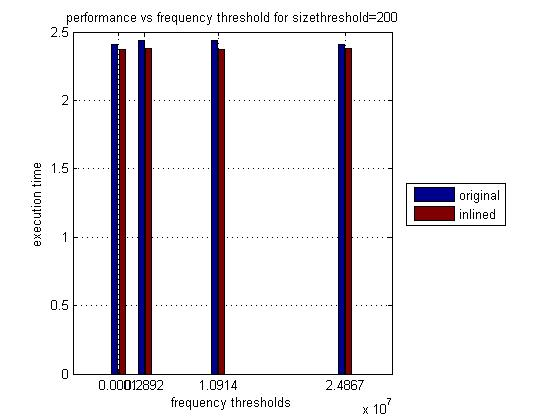
\includegraphics[width=0.25\textwidth]{cj_ft-time4.jpg}
        		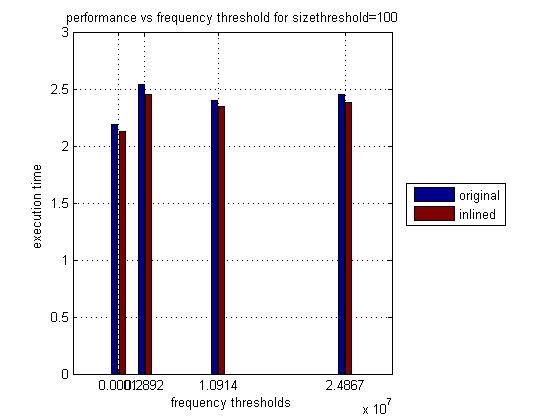
\includegraphics[width=0.25\textwidth]{cj_ft-time5.jpg}&
		\end{tabular}
	 \label{cj_ft_time}\caption{performance vs frequency threshold for cjson}
 \end{figure}

 \begin{figure}
	\centering
        \begin{tabular}{cc}
		    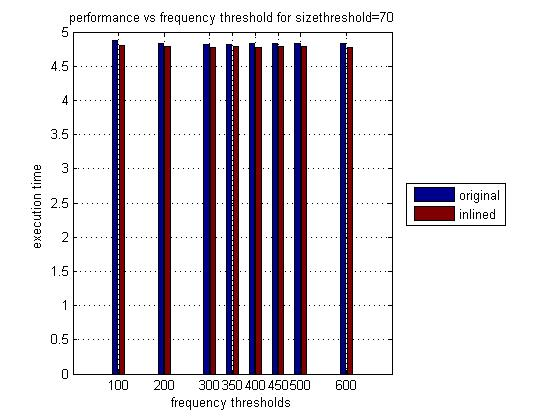
\includegraphics[width=0.25\textwidth]{pi_ft-time2.jpg}
		 	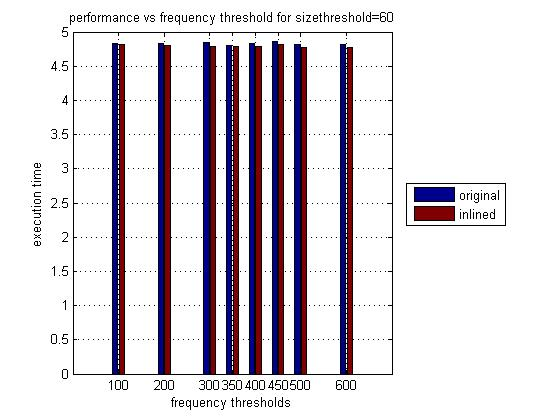
\includegraphics[width=0.25\textwidth]{pi_ft-time3.jpg}&
		\end{tabular}
	 \label{pi_ft_time}\caption{performance vs frequency threshold for pi.lua}
 \end{figure}

 \begin{figure}
	\centering
        \begin{tabular}{cc}
		 	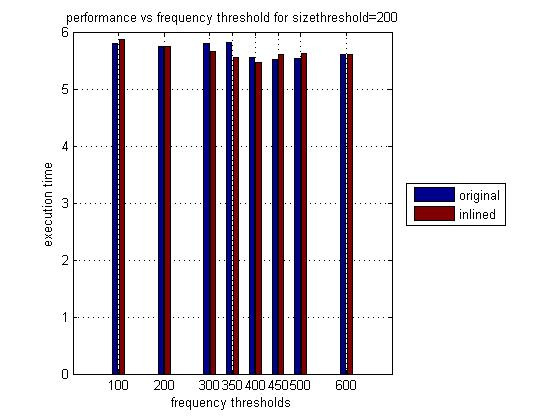
\includegraphics[width=0.25\textwidth]{src_ft-time4.jpg}
        		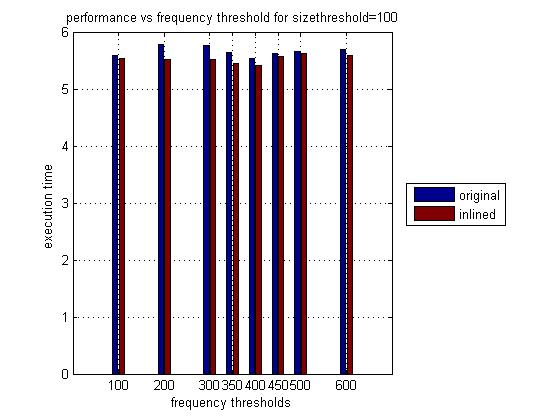
\includegraphics[width=0.25\textwidth]{src_ft-time5.jpg}&
		\end{tabular}
	 \label{src_ft_time}\caption{performance vs frequency threshold for src.lua}
 \end{figure}
 \begin{figure}
	 \begin{center}
		 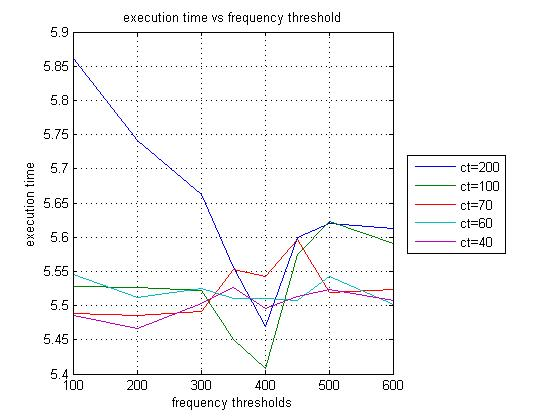
\includegraphics[width=0.5\textwidth]{src_analyser.jpg} 
	 \end{center}
	 \caption{exceution time vs frequency threshold for src.lua}
	 \label{src_ana}
 \end{figure}
 
 \begin{figure}
	 \begin{center}
		 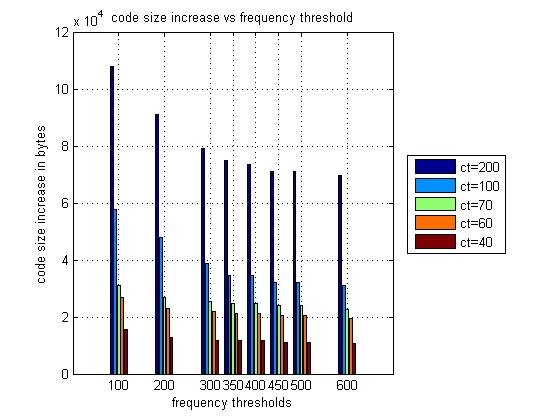
\includegraphics[width=0.5\textwidth]{codesizeincrease.jpg} 
	 \end{center}
	 \caption{exceution time vs frequency threshold for src.lua}
	 \label{src_cs}
 \end{figure}
 
 \begin{figure}
	 \begin{center}
		 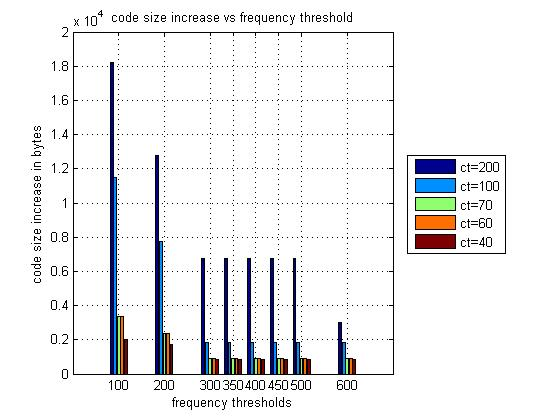
\includegraphics[width=0.5\textwidth]{pi_codesize.jpg} 
	 \end{center}
	 \caption{exceution time vs frequency threshold for pi.lua}
	 \label{pi_cs}
 \end{figure}
 
 \begin{figure}
	 \begin{center}
		 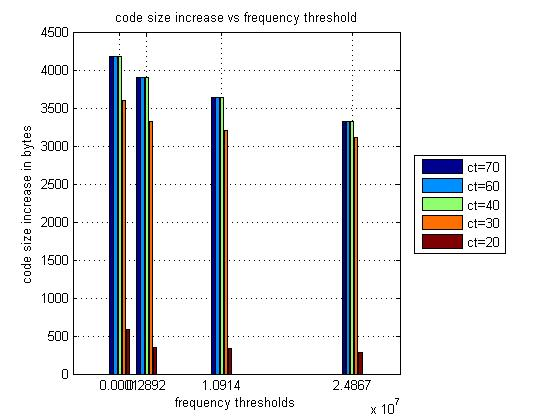
\includegraphics[width=0.5\textwidth]{cj_codesize.jpg} 
	 \end{center}
	 \caption{exceution time vs frequency threshold for cjson}
	 \label{cj_cs}
 \end{figure}

 
\subsection{Performance and Evaluation}
We run the above benchmarks on varying frequency threshold and minimum instruction count and examine the improvements [\ref{cj_ft_time},\ref{pi_ft_time},\ref{src_ft_time}]. Improvements grossly vary from 0.5-3\% . We also observe in \ref{src_ana} the code size growth with varying frequency thresholds[\ref{cj_cs} \ref{src_cs} \ref{pi_cs}]. An important observation from our frequency threshold vs performance graph[\ref{src_ana}] is that the frequency threshold where we get the highest performance is the one calculated by  our analyser thereby confirming its correctness atleast in the given benchmarks. The mere existence of the minima supports our assumption that an optimal frequency threshold does exist.
Apart from the above benchmark, we tested our implementation on a test code that had a huge number of mutators i.e. getter setter calls and could see a 9\% improvement in such codes.
All the performance data was calculated with an optimization level of 3 in LLVM i.e. the original bitcode file as well as the inlined bitcode file are both optimized before execution and the performance data is collected on this binary.  


\section{Conclusion and Future Work}
FDO based inlining approach gives at most 3\% improvement and on an average this approach gives 1.6\% improvement. However if the module contains various object mutators (like setter and getters) then those modules will be improved significantly. In those cases the developers do not have to use the inline keyword as the compiler will automatically detect those cases. Module containing the source code of the mutators has shown upto 10\% performance improvement on execution time. In those sense this process has some significant benefit. 
\paragraph*{•} The main problem with this approach is that we have to compile the whole program twice in order to get the optimal build. There is no process associated to this, which can make use of the knowledge, which it has gain by compiling similar type of programs. As we can see in the \cite{diego} work, there is a learning phase  associated to the optimization pass, similary  we can embrace some learning algorithm to optimize program for most general cases as future work and that will help us to get rid of the phase of repeated compiling of every program. There is one more direction in which this work can be extended, it is the cross module inlining optimization. Our cross module inling mechanis is very naive. Efficient cross module  analysis techniques, can help us to find more candidates for inlining.

\acks
We would like to thank Dr. Changhee Jung for his able guidance.

\bibliographystyle{abbrvnat}
\bibliography{report}
\end{document}

